%!TEX root=../main.tex
\section{Introduction}
Gaussian processes (GPs) are fully probabilistic models which can naturally estimate predictive uncertainty through posterior variances.
These uncertainties play a pivotal role in many application domains.
For example, uncertainty information is crucial when incorrect predictions could have catastrophic consequences, such as in medicine \cite{schulam2017if} or large-scale robotics \cite{deisenroth2015gaussian};
Bayesian optimization approaches typically incorporate model uncertainty when choosing actions \cite{snoek2012practical,deisenroth2011pilco,wang2017max};
and reliable uncertainty estimates are arguably useful for establishing trust in predictive models,
especially when predictions would be otherwise difficult to interpret
\cite{doshi2017roadmap,zhou2017effects}.

\emph{Although predictive uncertainties are a primary advantage of GP models, they have recently become their computational bottleneck.}
Historically, the use of GPs has been limited to problems with small datasets, since learning and inference computations na\"ively scale cubically with the number of data points ($n$).
Recent advances in \emph{inducing point methods} have managed to scale up GP training and computing predictive means to larger datasets \cite{snelson2006sparse,quinonero2005unifying,titsias2009variational}.
\emph{Kernel Interpolation for Scalable Structured GPs} (KISS-GP) is one such method that scales to millions of data points \cite{wilson2015kernel,wilson2015thoughts}.
For a test point $\bxtest$, KISS-GP expresses the predictive mean as $\bw_{\bxtest}^\top {\blue \ba'}$, where $\blue \ba'$ is a pre-computed vector dependent only on training data, and $\bw_\bxtest$ is a sparse interpolation vector.
This formulation affords the ability to compute predictive means in \emph{constant time}, independent of $n$.

\begin{figure}[t!]
  \centering
  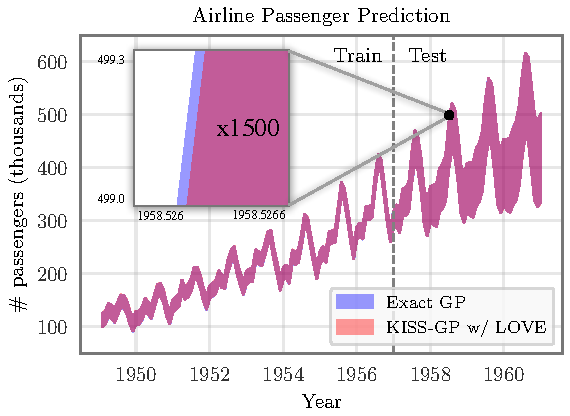
\includegraphics[width=0.8\columnwidth]{figures/airline_comparison.pdf}
  \caption{
    Comparison of predictive variances on airline passenger extrapolation.
    The variances predicted with LOVE{} are accurate within $10^{-4}$, yet can be computed orders of magnitude faster.
    \label{fig:airline_results}
  }
\end{figure}

However, these computational savings do not extend naturally to predictive uncertainties.
With KISS-GP, computing the predictive covariance between two points requires $\bigo{n + m \log m}$ computations, where $m$ is the number of inducing points (see \cref{tab:running_times}).
While this asymptotic complexity is lower than standard GP inference and alternative scalable approaches, it becomes prohibitive when $n$ is large, or when making many repeated computations.
Additionally, drawing samples from the predictive distributions -- a necessary operation in many applications -- is similarly expensive.
Existing fast approximations for these operations \cite{papandreou2011efficient,wilson2015thoughts,wang2017max} typically incur a significant amount of error.
Matching the reduced complexity of predictive mean inference without sacrificing accuracy has remained an open problem.

\begin{table*}[t!]
  \caption{
    Asymptotic complexities of predictive (co)variances ($N$ training points, $M$ inducing points, $J$ Lanczos/CG iterations)
    and sampling from the predictive distribution ($S$ samples, $T$ test points).
    \label{tab:running_times}
  }
  \vspace{0.5ex}
  \centering
  \resizebox{\textwidth}{!}{%
    \begin{tabular}{ |c||c|c||c||c| }
  \hline
  \multirow{2}*{\bf Method} & \multicolumn{2}{c||}{\bf Pre-computation}  & {\bf Computing variances} & {\bf Drawing $s$ samples} \\
                            & \multicolumn{1}{c}{(time)} & (storage) & (time) & (time) \\
  \hhline{|=#=|=|=#=|}
  Standard GP
  & $\bigo{n^3}$
  & $\bigo{n^2}$
  & $\bigo{n^2}$
  & $\bigo{t n^2 + t^2 (n + s) + t^3}$
  \\
  SGPR
  & $\bigo{nm^2}$
  & $\bigo{m^2}$
  & $\bigo{m^2}$
  & $\bigo{t m^2 + t^2 (m + s) + t^3}$
  \\
  KISS-GP
  & --
  & --
  & $\bigo{k (n \! + \! m \log m)}$
  & $\bigo{k t (n \! + \! m \log m) \! + \! t^2 (m + s)  \! + \! t^3}$
  \\ \hline
  {\color{\ourmethodcolor} KISS-GP (w/ LOVE{})}
  & {\color{\ourmethodcolor}$\bigo{k (n \! + \! m \log m)}$}
  & {\color{\ourmethodcolor}$\bigo{km}$}
  & {\color{\ourmethodcolor}$\bigo{k}$}
  & {\color{\ourmethodcolor} $\bigo{k s (t + m)}$} \\
  \hline
\end{tabular}

  }
  \vspace{-2ex}
\end{table*}


In this paper, we provide a solution based on the tridiagonalization algorithm of \citet{lanczos1950iteration}.
Our method takes inspiration from KISS-GP's mean computations: we express the predictive covariance between $\bx^*_i$ and $\bx^{*}_j$ as
$\bw_{\bxtest_i}^\top \blue{\bC} \: \bw_{\bxtest_j}$,
where $\blue C$ is an $M \times M$ matrix dependent only on training data.
However, we take advantage of the fact that $\blue \bC$ affords fast matrix-vector multiplications (MVMs) and avoid explicitly computing the matrix.
Using the Lanczos algorithm, we can efficiently decompose $\blue \bC$ as two rank-$J$ matrices $\blue \bC \approx \blue{\bR \bR^{\top \prime}}$ in \emph{nearly linear time}.
After this one-time upfront computation, and due to the special structure of $\blue {\bR,\bR^\prime}$, all variances can be computed in \emph{constant time} -- $\bigo{J}$ -- per (co)variance entry.
We extend this method to sample from the predictive distribution at $T$ points in $\bigo{T + M}$ time -- independent of training dataset size.

We refer to this method as LanczOs Variance Estimates, or LOVE{} for short.\footnote{
  LOVE{} is implemented in the GPyTorch library.
  Examples are available at \url{http://bit.ly/gpytorch-examples}.
}
LOVE{} has the lowest asymptotic complexity for computing predictive (co)variances and drawing samples with GPs.
We empirically validate LOVE{} on seven datasets and find that it consistently provides substantial speedups over existing methods \emph{without sacrificing accuracy}.
Variances and samples are accurate to within four decimals, and can be computed \emph{up to 18,000 times faster.}
